\documentclass[12pt,a4paper,oneside]{report}
\usepackage{allianceproject}
\usepackage{listings}
\usepackage{xcolor}
\lstset{
  basicstyle=\ttfamily\small,
  breaklines=true,
  frame=single,
  backgroundcolor=\color{gray!10},
  keywordstyle=\color{blue}\bfseries,
  commentstyle=\color{green!60!black},
  stringstyle=\color{orange},
  inputencoding=utf8,
  extendedchars=true
}
\addbibresource{references.bib}
\graphicspath{{figures/}}

% ===================== PROJECT METADATA =====================
\projecttitle{Microproject 5: Secure Password Storage System}
\projecttype{Micro Project 5}
\coursecode{E1CSA311}
\degree{Bachelor of Technology}
\branch{Computer Science and Engineering}
\department{Department of Computer Science and Engineering}
\academicyear{2026--2027}
\monthyear{October 2026}
\supervisor{Dr. Ambairam Muthu Sivakrishna}{Assistant Professor}
\hod{Dr. Oswalt Manoj S}
\projectlogo{Alliance_University_Icon.png}
\studentrows{
Arya Utkarsh & 2411021060543 \\
Akshat Kishore & 2411021060555 \\
D Sai Shikhar Achari & 2411021060542 \\
Joshua K R & 2411021060531 \\
}
% ============================================================

\begin{document}
\AllianceCoverPage
\AllianceFrontMatter
\AllianceTitlePage
\AllianceCertificate
\AllianceDeclaration

\AllianceAcknowledgement{%
We express our sincere gratitude to our supervisor, \AUSupervisor, for continuous guidance, technical feedback, and encouragement throughout this micro project. We also thank the Head of the Department, the project coordinators, reviewers, and faculty members of the Alliance School of Advanced Computing for their valuable suggestions and support. We acknowledge Alliance University for providing the academic environment and computing resources required for this work. Finally, we thank our peers, friends, and families for their encouragement and support.
}

\AllianceAbstract{Storing passwords securely is one of the most fundamental challenges in software security. Naive approaches such as plaintext storage or reversible encryption expose every user credential when a database is breached. This project presents and implements a local academic authentication system that demonstrates best-practice password storage using SHA-256 with unique random salts. Each password is concatenated with a 16-byte cryptographically random salt and passed through the SHA-256 hash function, producing a 32-byte (256-bit) irreversible digest. A constant-time HMAC comparison is used during verification to prevent timing side-channel attacks. Session tokens are independently hashed with plain SHA-256 before database storage. The system is implemented entirely in Python using only the standard library, with an SQLite backend, CSRF protection, rate limiting, and a live security dashboard that displays the actual stored salt and hash for each authenticated user. This design allows students to observe cryptographic principles in operation---the hash function, salt uniqueness, and one-way verification---without requiring any third-party packages. The project demonstrates that strong password protection is achievable with widely available primitives when they are composed correctly.}

\tableofcontents\clearpage
\listoftables\addcontentsline{toc}{chapter}{List of Tables}\clearpage
\listoffigures\addcontentsline{toc}{chapter}{List of Figures}\clearpage
\begin{abbreviations}
SHA  & Secure Hash Algorithm\\
HMAC & Hash-based Message Authentication Code\\
CSRF & Cross-Site Request Forgery\\
SQLite & Self-contained, serverless relational database engine\\
HTTP & Hypertext Transfer Protocol\\
HTTPS & HTTP Secure\\
TLS & Transport Layer Security\\
PBKDF2 & Password-Based Key Derivation Function 2\\
MAD & Median Absolute Deviation (mentioned for comparison)\\
UI & User Interface\\
API & Application Programming Interface\\
\end{abbreviations}

\AllianceMainMatter
\chapter{Introduction}
\label{chap:introduction}

\section{Background and Motivation}
\label{sec:intro_background}

Password-based authentication remains the most widely deployed mechanism for verifying user identity across web applications. Despite significant advances in multi-factor authentication and hardware security keys, the username-password pair continues to serve as the primary credential for the vast majority of online services. This ubiquity makes password storage one of the most consequential security decisions a developer makes: a single mistake at the storage layer can silently expose the credentials of every registered user in the event of a database breach.

History demonstrates the severity of such failures repeatedly. Large-scale breaches at major organisations have exposed hundreds of millions of password records, frequently revealing that even technology-savvy companies stored credentials without adequate cryptographic protection. Attackers who obtain a database dump can subsequently crack poorly protected passwords offline---at billions of guesses per second on commodity graphics hardware---without the victim organisation ever detecting the attack. The downstream consequences include credential-stuffing attacks against other services, financial fraud, and identity theft, all stemming from a deficiency in a single architectural decision.

This micro project addresses the educational dimension of the problem. While industry guidance from organisations such as the Open Web Application Security Project (OWASP) \cite{owasp2023} and the National Institute of Standards and Technology (NIST) \cite{nist2022} prescribes the use of adaptive hashing algorithms (bcrypt, scrypt, Argon2, PBKDF2), the underlying cryptographic principles---one-way functions, salting, and timing-safe comparison---are often opaque to students who have not yet encountered them in a concrete implementation context. This project bridges that gap by building a fully functional, self-contained authentication system in Python that makes the cryptographic machinery visible and inspectable through a live security dashboard.

\section{Problem Statement}
\label{sec:intro_problem}

Three classes of password-storage failure are particularly common in practice:

\begin{enumerate}
  \item \textbf{Plaintext storage.} Passwords are recorded verbatim in the database. Any individual with read access to the data store---a malicious insider, a misconfigured backup, or an attacker who exploits a SQL-injection vulnerability---immediately possesses all user credentials. This approach provides zero protection.

  \item \textbf{Unsalted or weakly-salted hashing.} Applying a cryptographic hash function (MD5, SHA-1, or even SHA-256) directly to a password without a unique, random salt allows precomputed rainbow-table attacks. An attacker who has built or downloaded a table mapping common passwords to their hashes can identify matching entries in the stolen database in milliseconds, regardless of how many users share the same password.

  \item \textbf{Fast, unadapted hash functions.} Even when a unique salt is used, employing a single iteration of a general-purpose hash such as MD5 or SHA-256 leaves the system vulnerable to brute-force search. Modern GPUs can evaluate billions of SHA-256 computations per second, making exhaustive search over large password spaces feasible in hours rather than years.
\end{enumerate}

This project directly addresses the first two failure modes through salted SHA-256 with constant-time verification, and explicitly discusses the third as a limitation motivating the use of adaptive key-derivation functions in production deployments.

\section{Approach and Contributions}
\label{sec:intro_approach}

The Secure Password Storage system demonstrates best-practice fundamentals using the following design choices:

\begin{itemize}
  \item \textbf{Unique random salts.} Each password registration generates 16 cryptographically random bytes (128 bits of entropy) via \texttt{secrets.token\_bytes}. The salt is concatenated with the UTF-8 encoded password before hashing, ensuring that two users with identical passwords produce distinct stored values, and eliminating the utility of precomputed rainbow tables.

  \item \textbf{SHA-256 one-way hashing.} The salted password data is processed by the SHA-256 compression function, producing a 256-bit irreversible digest. The stored credential record contains only the salt and the hash---never the raw password.

  \item \textbf{Constant-time comparison.} Password verification uses \texttt{hmac.compare\_digest}, which performs comparison in time proportional to the length of the strings rather than the position of the first differing byte. This eliminates the timing side-channel that would otherwise allow an attacker to make inferences about the stored hash by measuring response-time variations.

  \item \textbf{Session-token hashing and CSRF protection.} Session tokens are hashed with SHA-256 before database storage, so a database read does not yield usable tokens. CSRF tokens are generated using HMAC-SHA256 bound to the session identifier, providing request-forgery protection for all state-changing endpoints.

  \item \textbf{Rate limiting and account lockout.} A rolling 5-minute window limits failed login attempts to prevent online brute-force attacks.
\end{itemize}

The primary contributions of this project are:

\begin{enumerate}
  \item A complete, dependency-free Python implementation of salted SHA-256 password hashing with constant-time verification.
  \item A live security dashboard that renders the stored salt and hash for each authenticated user, making cryptographic principles directly observable.
  \item A comprehensive integration test suite (17 tests) that validates all security properties, including the absence of plaintext in the database and salt rotation on password change.
  \item A reproducible academic demonstration environment requiring only Python~3.10 and no external packages.
\end{enumerate}

\section{Report Organisation}
\label{sec:intro_organisation}

The remainder of this report is structured as follows. Chapter~\ref{chap:literature} surveys the history of password storage mechanisms and identifies the educational gap this project addresses. Chapter~\ref{chap:theory} provides theoretical background on SHA-256, salting, timing-safe comparison, and related security mechanisms, together with the system's functional and non-functional requirements. Chapter~\ref{chap:methodology} describes the proposed methodology and system design, including algorithm specifications and database schema. Chapter~\ref{chap:implementation} details the implementation and experimental setup. Chapter~\ref{chap:results} presents results and a security analysis. Chapter~\ref{chap:conclusion} concludes with lessons learned and directions for future work.

\chapter{Literature Review and Gap Analysis}
\label{chap:literature}

\section{Early Password Storage Mechanisms}
\label{sec:lit_early}

The history of password storage in computing systems stretches back to the origins of multi-user operating systems in the 1960s and 1970s. Early UNIX systems stored passwords in a world-readable \texttt{/etc/passwd} file, initially in plaintext and later using the DES-based \texttt{crypt(3)} function. The \texttt{crypt} scheme applied a modified DES cipher to a constant zero-block using the password as the key, iterated 25 times to slow computation, and encoded the result alongside a 12-bit salt. While this represented a significant conceptual advance---introducing both one-way transformation and a salt to defeat precomputation---the 8-character password limit imposed by DES key-scheduling and the rapid growth in computational power eventually made brute-force attacks against even salted \texttt{crypt} hashes tractable.

The fundamental insight of that era---that passwords should not be stored in recoverable form and that salts prevent two users with the same password from having identical records---remains valid today. What has changed is the computational gap between defenders and attackers: hardware improvements that once required decades to close can now be exploited in hours using commodity GPUs.

\section{The MD5 and SHA-1 Era: Failures in Practice}
\label{sec:lit_md5}

With the widespread adoption of the Internet in the 1990s and early 2000s, web applications proliferated and password databases became attractive targets. Many developers turned to general-purpose cryptographic hash functions---primarily MD5 and SHA-1---as convenient replacements for \texttt{crypt}. These functions are fast, standardised, and produce fixed-length outputs, making them superficially attractive for password storage. However, their use introduced two categories of vulnerability.

\subsection{Rainbow-Table Attacks}
\label{sec:lit_rainbow}

A rainbow table is a precomputed data structure that maps hash values to the passwords that produce them, exploiting a time-memory trade-off to recover passwords faster than online brute-force. When passwords are hashed without salts, an attacker need only compute the table once and can then look up any matching hash in the stolen database instantly. Rainbow tables for MD5-hashed passwords covering all alphanumeric strings up to eight characters have been publicly available for over two decades. Deployments that applied MD5 without salts were, in practice, storing recoverable passwords.

\subsection{Collision and Preimage Attacks}
\label{sec:lit_collision}

Beyond rainbow tables, MD5 was found to be fundamentally broken from a cryptographic standpoint. Wang and Yu demonstrated practical MD5 collisions in 2004, and MD5 was subsequently deprecated for all security-sensitive applications \cite{kelsey2005}. SHA-1 followed a similar trajectory: theoretical collision attacks were shown in 2005, and practical chosen-prefix collisions were demonstrated by the SHAttered project in 2017. While collision resistance is a distinct property from preimage resistance (the property relevant to password hashing), the widespread academic consensus against MD5 and SHA-1 led practitioners to migrate to SHA-2 family functions. SHA-256, the 256-bit member of SHA-2, remains collision-resistant and preimage-resistant to the best of current knowledge.

\section{Salted Hashes and Their Improvement}
\label{sec:lit_salted}

The introduction of per-user random salts substantially raised the bar against precomputed attacks. When each password record includes a unique salt, an attacker who obtains a database dump must crack each record independently; no precomputed table can span the full space of possible salted inputs. Early web frameworks such as Django (prior to its adoption of PBKDF2) used simple salted SHA-256, which provided meaningful protection against rainbow tables while remaining easy to implement. This approach---exactly the approach taken in the present project---is sufficient to demonstrate the core educational principles of one-way hashing and salt uniqueness.

However, salted SHA-256 without iteration retains a critical weakness: a single SHA-256 evaluation takes approximately 200--300 nanoseconds on a modern processor, meaning a GPU cluster can evaluate billions of candidates per second against a stolen hash. A determined attacker with knowledge of the salt can still mount an offline brute-force attack at enormous scale. This observation motivates the key-derivation functions discussed in the following section.

\section{Modern Key Derivation Functions}
\label{sec:lit_kdfs}

Contemporary guidance from OWASP \cite{owasp2023} and NIST \cite{nist2022} recommends password-specific key derivation functions (KDFs) that are deliberately slow and, in some cases, memory-hard. These functions are designed to require a configurable amount of computational work per evaluation, which can be increased over time to track improvements in attacker hardware.

\subsection{bcrypt}
\label{sec:lit_bcrypt}

Provos and Mazi\`{e}res introduced bcrypt in 1999 \cite{provos1999} as an adaptive hashing scheme based on the Blowfish block cipher. A \emph{cost factor} parameter controls the number of rounds of the expensive key-setup phase; doubling the cost factor doubles the time required per hash. bcrypt has been widely adopted in web frameworks and remains a recommended choice for password hashing when memory-hardness is not required. Its primary limitation is a 72-byte maximum effective password length imposed by Blowfish key scheduling.

\subsection{scrypt}
\label{sec:lit_scrypt}

Percival introduced scrypt in 2009 \cite{percival2009} as a sequential memory-hard function designed to impose both time and memory costs. By requiring the evaluator to read from a large, pseudo-randomly addressed memory buffer, scrypt ensures that parallelisation using ASICs or GPUs---which have limited memory bandwidth relative to their computational throughput---does not provide the attacker with an asymmetric advantage. scrypt forms the basis of several cryptocurrency proof-of-work schemes and is supported by Python's \texttt{hashlib} module.

\subsection{Argon2}
\label{sec:lit_argon2}

Argon2 \cite{biryukov2016}, the winner of the Password Hashing Competition in 2015, represents the current state of the art. It offers three variants: Argon2d (data-dependent, suitable for cryptocurrency), Argon2i (data-independent, suitable for password hashing in side-channel-sensitive environments), and Argon2id (a hybrid recommended by OWASP). Argon2 parameters include time cost, memory cost, and parallelism degree, providing flexible tuning for a wide range of deployment scenarios.

\subsection{PBKDF2}
\label{sec:lit_pbkdf2}

PBKDF2 (Password-Based Key Derivation Function 2), standardised in RFC 2898 and recommended by NIST SP 800-132, applies a pseudorandom function (typically HMAC-SHA256) to the password and salt iteratively. NIST SP 800-63B recommends at least 600,000 iterations of PBKDF2-HMAC-SHA256 for password hashing. Python's \texttt{hashlib} module exposes PBKDF2 via \texttt{hashlib.pbkdf2\_hmac}. While not memory-hard, PBKDF2 is widely supported and compliant with FIPS 140-2.

Table~\ref{tab:algo_comparison} summarises the key properties of the hash algorithms discussed above.

\begin{table}[H]
\centering
\caption{Comparison of hash algorithms for password storage}
\label{tab:algo_comparison}
\small
\begin{tabularx}{\textwidth}{|p{3.2cm}|c|c|p{2.8cm}|X|}
\hline
\textbf{Algorithm} & \textbf{Output} & \textbf{Collision Res.} & \textbf{Speed} & \textbf{Password Use} \\\hline
MD5       & 128 bits  & Broken          & Very fast ($>$1 GH/s) & No \\\hline
SHA-1     & 160 bits  & Broken          & Very fast             & No \\\hline
SHA-256   & 256 bits  & Strong          & Fast ($\sim$1 GH/s)   & Educational only \\\hline
PBKDF2-SHA256 & 256 bits & Strong       & Configurable          & Yes (NIST) \\\hline
bcrypt    & 192 bits  & Strong          & Configurable          & Yes (72-byte max) \\\hline
scrypt    & Variable  & Strong          & Memory-hard           & Yes \\\hline
Argon2id  & Variable  & Strong          & Time+Memory-hard      & Yes (OWASP Rec.) \\\hline
\end{tabularx}
\end{table}

\section{Comparison of Password Storage Schemes}
\label{sec:lit_schemes}

Beyond the choice of hash algorithm, the overall storage \emph{scheme} determines the practical security of the system. Table~\ref{tab:scheme_comparison} compares common schemes along four dimensions relevant to this project.

\begin{table}[H]
\centering
\caption{Comparison of password storage schemes}
\label{tab:scheme_comparison}
\begin{tabularx}{\textwidth}{|l|c|c|c|X|}
\hline
\textbf{Scheme} & \textbf{Salted} & \textbf{One-Way} & \textbf{Timing-Safe} & \textbf{Educational Value} \\\hline
Plaintext storage      & No  & No  & N/A & Low (trivially broken) \\\hline
MD5 (unsalted)         & No  & Yes & No  & Low (broken) \\\hline
SHA-256 (unsalted)     & No  & Yes & No  & Moderate (rainbow-table demo) \\\hline
Salted SHA-256         & Yes & Yes & Configurable & \textbf{High} (teaches core concepts) \\\hline
PBKDF2-HMAC-SHA256     & Yes & Yes & Yes & High (production-ready) \\\hline
bcrypt                 & Yes & Yes & Yes & High (widely deployed) \\\hline
Argon2id               & Yes & Yes & Yes & High (state-of-the-art) \\\hline
\end{tabularx}
\end{table}

\section{Gap Analysis}
\label{sec:lit_gap}

A survey of the existing literature and educational tools reveals a gap between two extremes. On one hand, introductory security textbooks explain salting and one-way hashing at a conceptual level without a hands-on implementation. On the other hand, production frameworks such as Django or Flask-Bcrypt abstract the cryptographic machinery behind high-level API calls, making it impossible for a student to observe the individual steps of salt generation, hash computation, and comparison. A live, inspectable demonstration application---one that renders the actual salt bytes and hash digest on screen for each authenticated user---addresses this gap directly.

Furthermore, no widely distributed, purely standard-library Python application exists that combines all five security properties in one codebase: salted SHA-256 hashing, constant-time comparison, CSRF protection, rate limiting, and session-token hashing. The present project fills this niche, providing a reproducible academic artefact that instructors can deploy in minutes and students can study, modify, and extend.

\chapter{Theoretical Background and Requirements}
\label{chap:theory}

\section{The SHA-256 Hash Function}
\label{sec:theory_sha256}

SHA-256 is a member of the Secure Hash Algorithm 2 (SHA-2) family, standardised by NIST in Federal Information Processing Standard (FIPS) 180-4. It maps an arbitrary-length bit string to a fixed-length 256-bit (32-byte) digest. Formally, the function is written as:

\begin{equation}
  H : \{0,1\}^{*} \to \{0,1\}^{256}
  \label{eq:sha256_domain}
\end{equation}

\noindent where $\{0,1\}^{*}$ denotes the set of all finite binary strings. For a message $m$, the hash is:

\begin{equation}
  d = H(m) = \mathrm{SHA\text{-}256}(m)
  \label{eq:sha256_notation}
\end{equation}

\subsection{Internal Structure}
\label{sec:theory_sha256_internal}

SHA-256 processes input in 512-bit (64-byte) blocks through a Merkle--Damg\r{a}rd construction. The message $m$ is first padded to a length congruent to $448 \pmod{512}$ bits, and the 64-bit big-endian representation of the original message length is appended to produce a padded message $m'$ of length $N \times 512$ bits. The function then iterates a compression function $f$ over each block:

\begin{equation}
  s_0 = H_0, \qquad s_i = f(s_{i-1}, B_i) \text{ for } i = 1, \ldots, N, \qquad d = s_N
  \label{eq:sha256_merkle}
\end{equation}

\noindent where $H_0$ is a 256-bit initialisation vector derived from the fractional parts of the square roots of the first eight primes, $B_i$ is the $i$-th 512-bit block, and $s_N$ is the final digest. The compression function $f$ uses 64 rounds of bitwise operations (choice, majority, sigma rotations) and 64 round constants derived from the fractional parts of the cube roots of the first 64 primes.

\subsection{Security Properties}
\label{sec:theory_sha256_properties}

SHA-256 provides three fundamental security properties relevant to password hashing:

\begin{itemize}
  \item \textbf{Preimage resistance.} Given a digest $d$, it is computationally infeasible to find any $m$ such that $H(m) = d$. This ensures that an attacker who obtains a stored hash cannot reverse it to recover the password. The best known preimage attack against the full SHA-256 requires approximately $2^{256}$ operations---far beyond any feasible computation.

  \item \textbf{Second preimage resistance.} Given a message $m_1$, it is computationally infeasible to find a distinct $m_2$ such that $H(m_1) = H(m_2)$. This property ensures that knowledge of one input does not allow construction of a colliding input.

  \item \textbf{Collision resistance.} It is computationally infeasible to find any two distinct messages $m_1 \neq m_2$ such that $H(m_1) = H(m_2)$. The best known collision attacks against SHA-256 have complexity approximately $2^{128}$ by the birthday bound, which remains computationally infeasible.

  \item \textbf{Avalanche effect.} A single-bit change in the input produces, on average, a change in approximately 50\% of the output bits, making it impossible to infer any information about the input from partial knowledge of the output.
\end{itemize}

\section{Salting}
\label{sec:theory_salting}

A \emph{salt} is a random value generated independently for each stored password record and prepended (or appended) to the password before hashing. In this system, a 16-byte (128-bit) salt is generated using Python's \texttt{secrets.token\_bytes(16)}, which draws from the operating-system cryptographically secure pseudorandom number generator (CSPRNG).

\subsection{Defeating Rainbow Tables}
\label{sec:theory_rainbow}

A rainbow table attack exploits the fact that if two users choose the same password, their unsalted hashes are identical, and a precomputed table can reveal both simultaneously. With unique salts, the effective input to the hash function for each record is:

\begin{equation}
  \text{input}_i = s_i \| p
  \label{eq:salted_input}
\end{equation}

\noindent where $s_i$ is the per-user 128-bit random salt and $p$ is the password as a UTF-8 byte string. The stored credential is then:

\begin{equation}
  \text{stored}_i = H(s_i \| p) = \mathrm{SHA\text{-}256}(s_i \| p)
  \label{eq:salted_hash}
\end{equation}

Because $s_i$ is chosen uniformly at random from a $2^{128}$-element space, no precomputed table can cover even a negligible fraction of the possible salted inputs. An attacker must crack each record individually, starting the hash computation from scratch for each candidate password.

\subsection{Salt Uniqueness and Storage}
\label{sec:theory_salt_storage}

The salt must be stored alongside the hash so that verification can reproduce the exact salted input. In this project the salt and hash are stored together in an encoded string:

\begin{equation}
  \text{encoded} = \texttt{"sha256\$"} \| \mathrm{hex}(s) \| \texttt{"\$"} \| \mathrm{hex}(H(s \| p))
  \label{eq:encoded_format}
\end{equation}

\noindent This format is self-describing: the algorithm identifier, salt, and hash are separated by \texttt{\$} delimiters, allowing the \texttt{verify\_password} function to parse all required fields from a single string without additional database columns.

\section{Constant-Time Comparison and Timing Side-Channels}
\label{sec:theory_timing}

Password verification involves comparing the recomputed hash against the stored hash. A naive implementation using Python's built-in string equality operator (\texttt{==}) terminates as soon as the first differing byte is found, producing a response time that is inversely correlated with the length of the common prefix. An attacker who can measure server response time with sufficient precision can exploit this variation---submitting crafted hashes and observing which ones take slightly longer---to reconstruct the stored hash one byte at a time. This is a \emph{timing side-channel attack}.

The countermeasure is a \emph{constant-time comparison}: a comparison that always examines every byte of both operands, regardless of where the first difference occurs. Python's standard library provides this via \texttt{hmac.compare\_digest(a, b)}, which is implemented in C and guaranteed to run in time $O(|a|)$ independent of the content of $a$ and $b$. Formally, for two byte strings $a$ and $b$ of the same length $n$:

\begin{equation}
  \mathrm{compare\_digest}(a, b) = \left(\bigoplus_{i=1}^{n} (a_i \oplus b_i)\right) = 0
  \label{eq:constant_time}
\end{equation}

\noindent where $\oplus$ denotes XOR. The result is \texttt{True} if and only if all bytes are identical, and the execution time is independent of the content.

\section{CSRF Tokens and HMAC}
\label{sec:theory_csrf}

Cross-Site Request Forgery (CSRF) is an attack in which a malicious web page causes the victim's browser to submit an authenticated request to a target site without the user's knowledge. The standard countermeasure is a \emph{synchroniser token}: a secret value bound to the user's session that must be submitted with every state-changing request and that a third-party site cannot obtain.

In this project, CSRF tokens are generated using HMAC-SHA256:

\begin{equation}
  \tau = \mathrm{HMAC\text{-}SHA256}(k_{\text{session}},\; \texttt{"csrf"})
  \label{eq:csrf_token}
\end{equation}

\noindent where $k_{\text{session}}$ is the raw (pre-storage) session token. The HMAC construction guarantees that the token is unpredictable without knowledge of the session secret, and that it changes with each new session. Because the HMAC key is never transmitted to the client, a cross-origin page cannot forge a valid token.

\section{Rate Limiting}
\label{sec:theory_rate}

Rate limiting protects against online brute-force attacks by capping the number of authentication attempts an attacker can make in a given time window. This project implements a bucket-based rate limiter with a 5-minute rolling window: at most 5 failed login attempts are permitted per username per 5-minute period. A failed attempt increments the attempt counter and records the timestamp; successful login resets the counter; and any request arriving when the counter has reached its limit is rejected with an error response before the hash comparison is performed.

\section{Session Management}
\label{sec:theory_sessions}

Session tokens are 32-byte values generated by the CSPRNG. Before storage in the database, each token is hashed with SHA-256:

\begin{equation}
  t_{\text{stored}} = \mathrm{SHA\text{-}256}(t_{\text{raw}})
  \label{eq:session_hash}
\end{equation}

\noindent The raw token is delivered to the client in an \texttt{HttpOnly; SameSite=Lax} cookie. Because the database stores only the hash, a database read does not yield a usable session token, limiting the damage from database compromise. On password change, all existing session records for the user are deleted, forcing re-authentication on all devices.

\section{System Requirements}
\label{sec:theory_requirements}

\subsection{Functional Requirements}
\label{sec:theory_func_req}

\begin{enumerate}
  \item \textbf{FR-1: User Registration.} The system shall accept a username and password, validate the username format (alphanumeric, 3--32 characters), enforce a minimum password length of 8 characters, generate a unique random salt, compute a salted SHA-256 hash, and store the encoded credential in the database.

  \item \textbf{FR-2: User Login.} The system shall accept a username and password, retrieve the stored encoded credential, recompute the salted hash, perform a constant-time comparison, and either issue a new session token or return a generic error message without revealing whether the username or password was incorrect.

  \item \textbf{FR-3: Password Change.} The system shall allow an authenticated user to change their password, requiring the current password for confirmation, generating a new salt, computing a new hash, revoking all existing sessions, and persisting the updated credential.

  \item \textbf{FR-4: Logout.} The system shall allow an authenticated user to invalidate their current session, removing the session token from both the client cookie and the server database.

  \item \textbf{FR-5: Security Dashboard.} The system shall display the stored salt (hex-encoded) and stored hash (hex-encoded) for the authenticated user's account, making the cryptographic artefacts directly observable.
\end{enumerate}

\subsection{Non-Functional Requirements}
\label{sec:theory_nonfunc_req}

\begin{enumerate}
  \item \textbf{NFR-1: No Plaintext Storage.} The database must contain no recoverable representation of any user's password. All integration tests must verify this property by reading the raw SQLite records.

  \item \textbf{NFR-2: Timing Safety.} All hash comparisons must use constant-time primitives. Response time must not vary with the content of the submitted password or the stored hash.

  \item \textbf{NFR-3: CSRF Protection.} All POST requests that modify server state (register, login, change password, logout) must include a valid CSRF token. Requests without a valid token must be rejected with HTTP 403.

  \item \textbf{NFR-4: Rate Limiting.} At most 5 failed login attempts per username per 5-minute window must be enforced. Requests exceeding this limit must be rejected before hash computation.

  \item \textbf{NFR-5: No External Dependencies.} The application must run using only the Python 3.10 standard library. No \texttt{pip install} step must be required.

  \item \textbf{NFR-6: Salt Uniqueness on Change.} When a user changes their password, a new salt must be generated. The old salt must not be reused.
\end{enumerate}

\chapter{Proposed Methodology and System Design}
\label{chap:methodology}

\section{Overall System Architecture}
\label{sec:arch_overview}

The application follows a layered architecture in which each layer has a single, well-defined responsibility. Figure~\ref{fig:architecture} depicts the high-level data flow.

\begin{figure}[H]
\centering
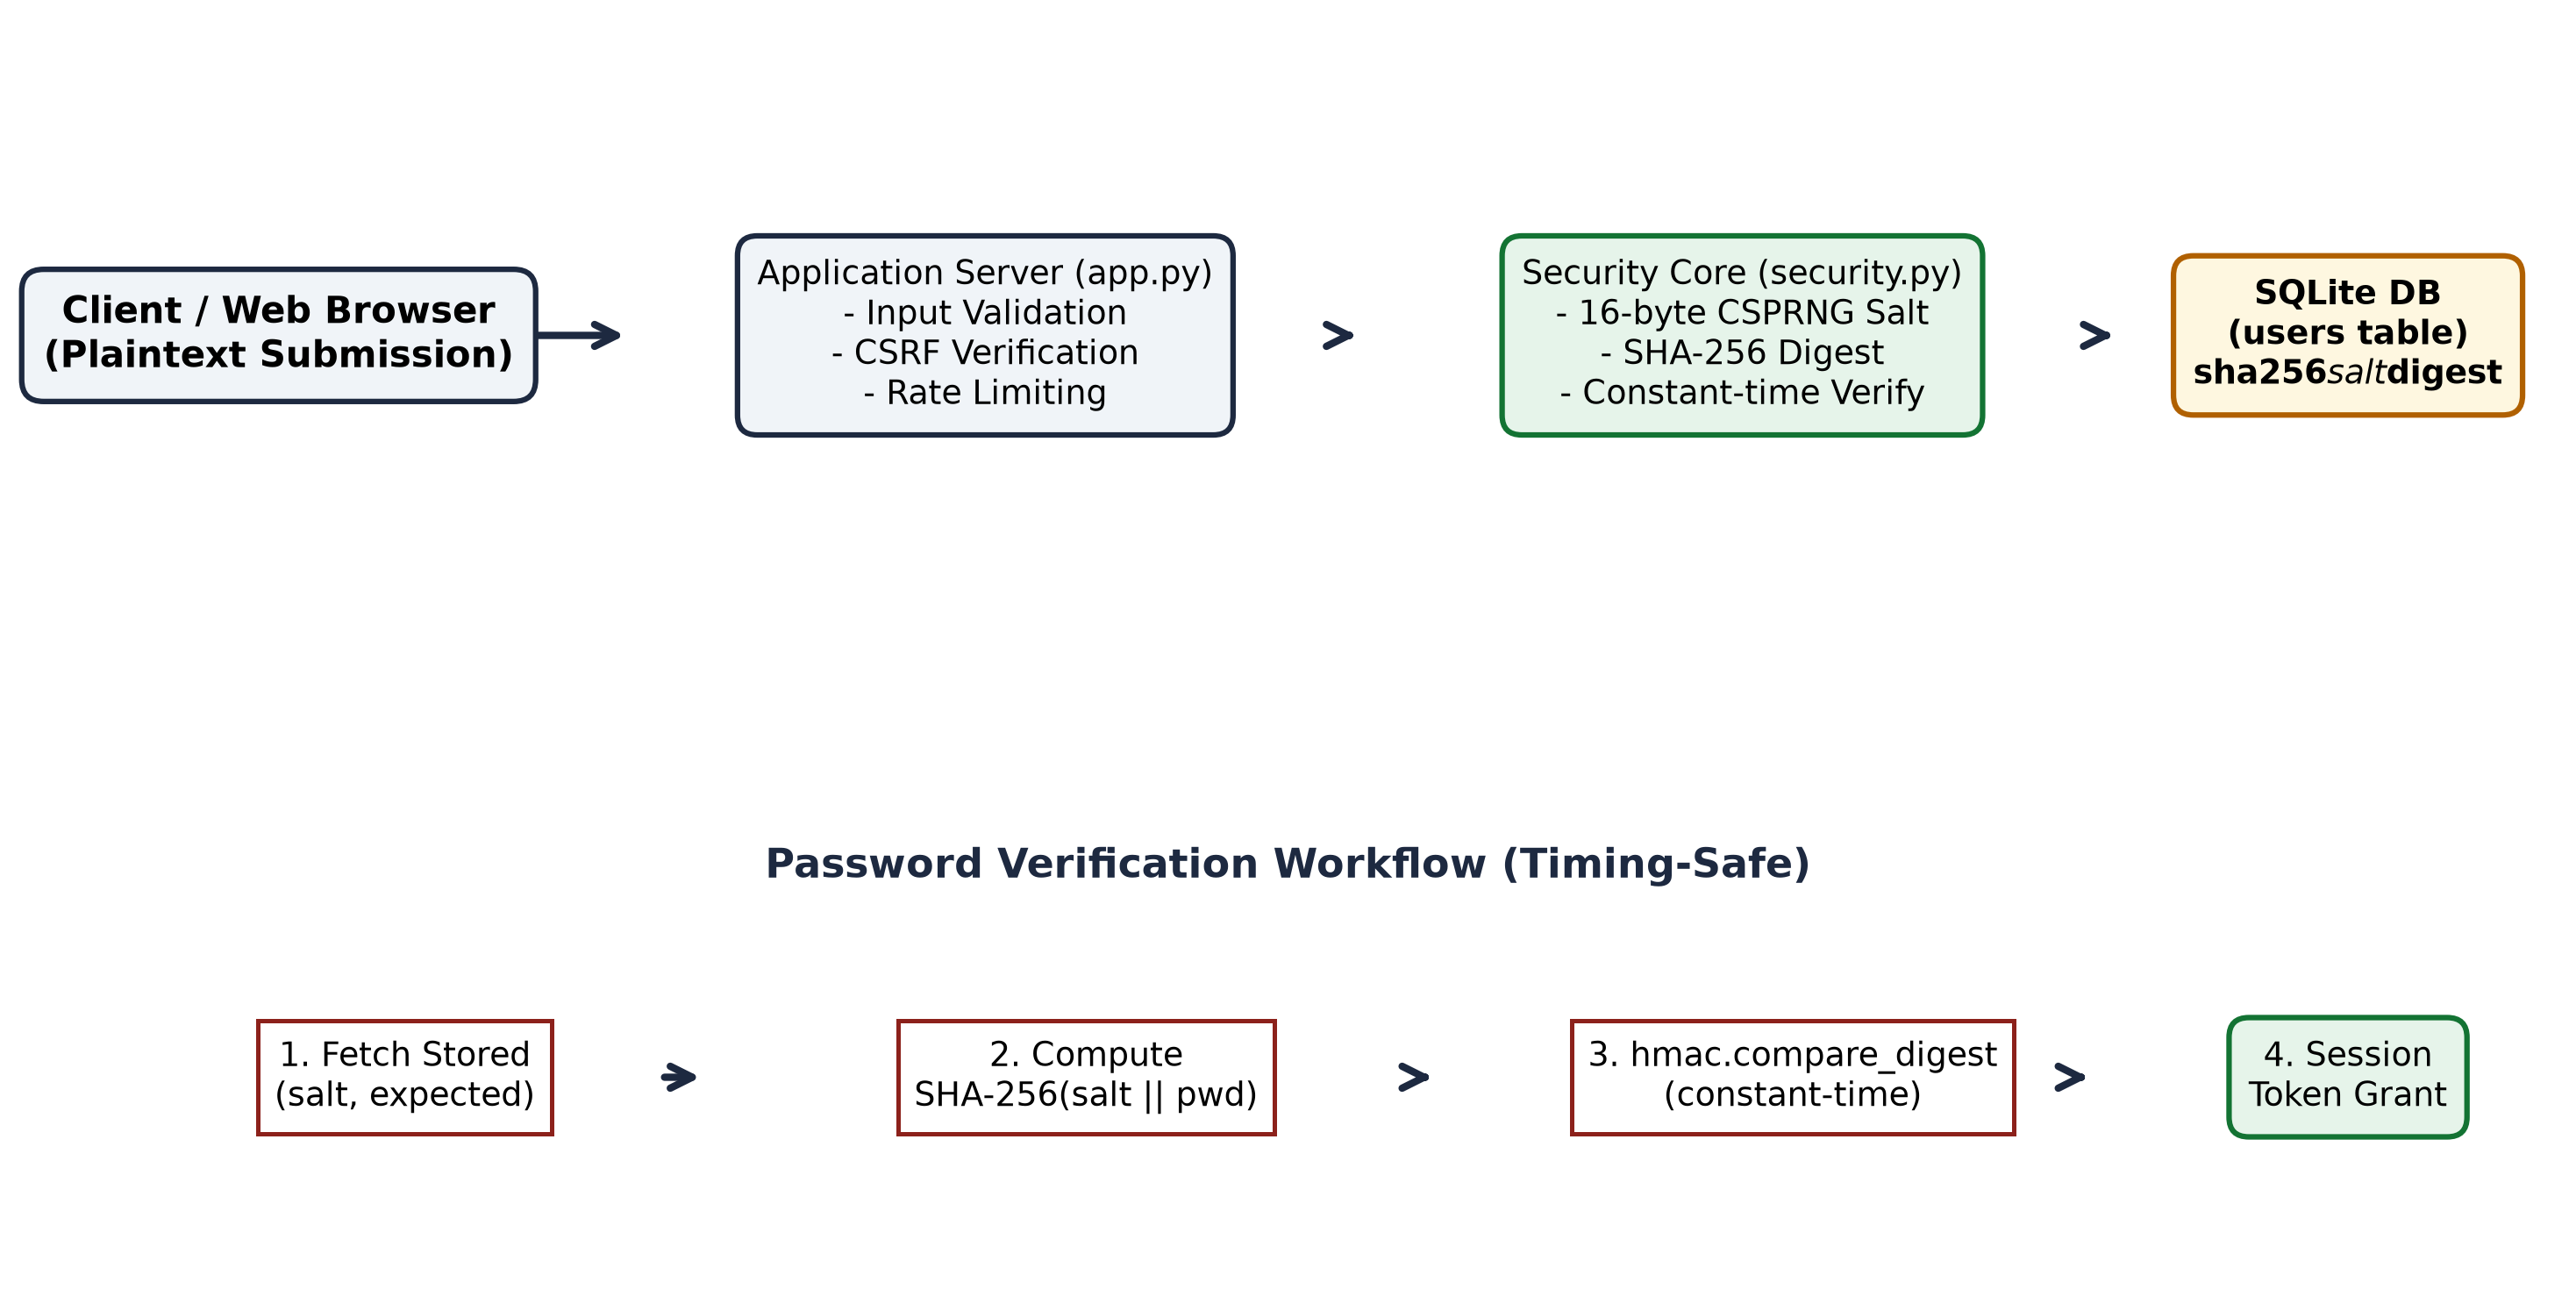
\includegraphics[width=0.95\textwidth]{architecture.png}
\caption{High-level system architecture showing layered data flow and verification workflow}
\label{fig:architecture}
\end{figure}

\begin{itemize}
  \item \textbf{Browser.} The client renders HTML pages served by the application and submits forms via HTTP POST. All cookies are \texttt{HttpOnly} and \texttt{SameSite=Lax} to mitigate XSS-based cookie theft and CSRF.

  \item \textbf{HTTP Handler (\texttt{app.py}).} A subclass of Python's \texttt{http.server.BaseHTTPRequestHandler} routes incoming requests, parses form data and cookies, enforces CSRF tokens, invokes rate limiting, delegates to the crypto layer for hash computation, and writes HTML responses.

  \item \textbf{Crypto Layer (\texttt{security.py}).} Contains all cryptographic operations: salt generation, SHA-256 hashing, constant-time comparison, session token generation, and CSRF token generation/validation using HMAC-SHA256.

  \item \textbf{Database Layer (\texttt{database.py}).} Wraps SQLite operations. All SQL statements use parameterised queries to eliminate SQL-injection risk. The layer exposes typed Python functions (not raw SQL) to the HTTP handler.

  \item \textbf{SQLite.} Stores the four tables described in Section~\ref{sec:arch_schema}. Never stores a password, session token, or any other secret in recoverable form.
\end{itemize}

\section{Cryptographic Module Design}
\label{sec:arch_crypto}

\subsection{The \texttt{hash\_password} Function}
\label{sec:arch_hash}

The primary credential-generation function accepts a plaintext password string and returns a self-describing encoded string containing the algorithm identifier, the hexadecimal salt, and the hexadecimal digest. The design steps are:

\begin{enumerate}
  \item \textbf{Salt generation.} Sixteen bytes are drawn from the OS CSPRNG via \texttt{secrets.token\_bytes(16)}, providing 128 bits of entropy. This salt is unique per registration event (or per password-change event).

  \item \textbf{Input construction.} The salt bytes are concatenated with the UTF-8 encoding of the password: $\text{data} = s \| \mathrm{encode}(p)$. This ensures that the hash function receives the full salted input as a single byte string, avoiding any ambiguity from separate HMAC-style key and data arguments.

  \item \textbf{Hash computation.} Python's \texttt{hashlib.sha256(data).digest()} computes the 32-byte SHA-256 digest in one call.

  \item \textbf{Encoding.} The encoded credential is assembled as: \newline
    \texttt{"sha256\$" + salt.hex() + "\$" + digest.hex()} \newline
    This yields a 32-character salt field and a 64-character digest field, separated by \texttt{\$} delimiters and prefixed by the algorithm name, for a total string length of approximately 103 characters.
\end{enumerate}

Algorithm~\ref{alg:hash_password} presents this logic in pseudocode.

\begin{algorithm}[H]
\caption{hash\_password($p$)}
\label{alg:hash_password}
\KwInput{Password string $p$}
\KwOutput{Encoded credential string}
$s \leftarrow \mathrm{CSPRNG}(16)$ \tcp*{16 random bytes}
$\text{data} \leftarrow s \;\|\; p.\mathrm{encode}(\texttt{utf-8})$\;
$d \leftarrow \mathrm{SHA\text{-}256}(\text{data})$\;
\Return $\texttt{"sha256\$"} \| \mathrm{hex}(s) \| \texttt{"\$"} \| \mathrm{hex}(d)$\;
\end{algorithm}

\subsection{The \texttt{verify\_password} Function}
\label{sec:arch_verify}

Password verification reconstructs the salted hash from the stored encoded string and compares it with the hash of the candidate password. Algorithm~\ref{alg:verify_password} details the procedure.

\begin{algorithm}[H]
\caption{verify\_password($p$, encoded)}
\label{alg:verify_password}
\KwInput{Candidate password $p$; encoded credential string}
\KwOutput{Boolean (True if password matches)}
Parse $\text{encoded}$ into $(\text{alg}, s_{\text{hex}}, d_{\text{hex}})$ by splitting on \texttt{"\$"}\;
\If{$\text{alg} \neq \texttt{"sha256"}$ \textbf{or} $|\text{parts}| \neq 3$}{
    \Return \textbf{False}\;
}
$s \leftarrow \mathrm{bytes.fromhex}(s_{\text{hex}})$\;
$d_{\text{expected}} \leftarrow \mathrm{bytes.fromhex}(d_{\text{hex}})$\;
$\text{data} \leftarrow s \;\|\; p.\mathrm{encode}(\texttt{utf-8})$\;
$d_{\text{actual}} \leftarrow \mathrm{SHA\text{-}256}(\text{data})$\;
\Return $\mathrm{hmac.compare\_digest}(d_{\text{actual}},\; d_{\text{expected}})$\;
\end{algorithm}

The use of \texttt{hmac.compare\_digest} in the final step is essential: it guarantees that the comparison time is independent of the content of the digests, eliminating timing side-channels as described in Section~\ref{sec:theory_timing}.

\subsection{Session Token Hashing}
\label{sec:arch_session_tokens}

Session tokens are 32-byte values produced by \texttt{secrets.token\_bytes(32)}. Before insertion into the \texttt{sessions} table, each token is hashed:

\begin{equation}
  t_{\text{stored}} = \mathrm{SHA\text{-}256}(t_{\text{raw}})
  \label{eq:session_token_hash}
\end{equation}

The raw token is placed in the client's \texttt{session\_id} cookie. During request handling, the handler hashes the incoming cookie value and queries the \texttt{sessions} table for a matching \texttt{token\_hash}. This ensures that compromise of the database does not yield usable session identifiers.

\subsection{CSRF Token Generation and Validation}
\label{sec:arch_csrf}

CSRF tokens are generated on login and stored in both the session record and an \texttt{HttpOnly} cookie. They are produced as:

\begin{equation}
  \tau = \mathrm{HMAC\text{-}SHA256}(t_{\text{raw}},\; \texttt{"csrf"}).\mathrm{hex}()
  \label{eq:csrf_generation}
\end{equation}

Every state-changing POST handler reads the CSRF token from the submitted form field and from the server-side session record, then compares them using \texttt{hmac.compare\_digest}. A mismatch returns HTTP~403 without performing any further processing.

\section{Database Schema}
\label{sec:arch_schema}

The SQLite database contains four tables. All tables use the \texttt{STRICT} keyword where supported to enforce column types.

\begin{table}[H]
\centering
\caption{Database schema: \texttt{users} table}
\label{tab:schema_users}
\begin{tabularx}{\textwidth}{|l|l|X|}
\hline
\textbf{Column} & \textbf{Type} & \textbf{Description} \\\hline
\texttt{id}              & INTEGER PRIMARY KEY & Auto-increment identifier \\\hline
\texttt{username}        & TEXT UNIQUE NOT NULL & Normalised lowercase username \\\hline
\texttt{password\_hash}  & TEXT NOT NULL & Encoded credential: \texttt{sha256\$<salt\_hex>\$<hash\_hex>} \\\hline
\texttt{created\_at}     & TEXT NOT NULL & ISO-8601 timestamp of registration \\\hline
\texttt{last\_login}     & TEXT & ISO-8601 timestamp of most recent successful login \\\hline
\end{tabularx}
\end{table}

\begin{table}[H]
\centering
\caption{Database schema: \texttt{sessions} table}
\label{tab:schema_sessions}
\begin{tabularx}{\textwidth}{|l|l|X|}
\hline
\textbf{Column} & \textbf{Type} & \textbf{Description} \\\hline
\texttt{id}            & INTEGER PRIMARY KEY & Auto-increment identifier \\\hline
\texttt{user\_id}      & INTEGER REFERENCES users & Foreign key to \texttt{users.id} \\\hline
\texttt{token\_hash}   & TEXT UNIQUE NOT NULL & SHA-256 of raw session token \\\hline
\texttt{csrf\_token}   & TEXT NOT NULL & HMAC-SHA256 CSRF token bound to session \\\hline
\texttt{expires\_at}   & TEXT NOT NULL & ISO-8601 expiry timestamp \\\hline
\texttt{created\_at}   & TEXT NOT NULL & ISO-8601 creation timestamp \\\hline
\end{tabularx}
\end{table}

\noindent The \texttt{attempts} table records failed login attempts (username, timestamp, IP address) to support rate limiting. The \texttt{activity} table records successful login and logout events for audit purposes.

\section{Rate Limiting Design}
\label{sec:arch_rate_limiting}

The rate limiter uses a bucket-based algorithm with a 5-minute rolling window. On each authentication attempt, the system:

\begin{enumerate}
  \item Queries the \texttt{attempts} table for all failed attempts by the given username in the past 300 seconds.
  \item If the count is $\geq 5$, the request is rejected with an HTTP 429 response before any hash computation is performed.
  \item If the authentication succeeds, all attempt records for that username are deleted (clearing the bucket).
  \item If the authentication fails, a new record is inserted into \texttt{attempts}.
\end{enumerate}

Importantly, the rate limiter runs \emph{before} the hash computation on failure paths, so it does not introduce a timing signal about the validity of the username. A ``dummy'' \texttt{verify\_password} call (computing \texttt{hash\_password("dummy")} and immediately discarding the result) is executed even when no matching user is found, ensuring that the response time for invalid usernames matches the response time for valid usernames with incorrect passwords.

\chapter{Implementation and Experimental Setup}
\label{chap:implementation}

\section{Development Environment}
\label{sec:impl_env}

The application is developed and tested on the following environment:

\begin{itemize}
  \item \textbf{Operating System:} macOS 14 Sonoma / Ubuntu 22.04 LTS (both supported).
  \item \textbf{Python Version:} CPython 3.10 or later (tested on 3.10, 3.11, 3.12).
  \item \textbf{External Dependencies:} None. All functionality is built exclusively from the Python standard library.
  \item \textbf{Standard Library Modules Used:} \texttt{http.server}, \texttt{hashlib}, \texttt{hmac}, \texttt{secrets}, \texttt{sqlite3}, \texttt{urllib.parse}, \texttt{http.cookies}, \texttt{datetime}, \texttt{json}, \texttt{unittest}.
  \item \textbf{Database:} SQLite 3.x (bundled with Python), stored at \texttt{data/securepassword.sqlite3}.
  \item \textbf{IDE:} Any text editor; no build system or compilation step required.
\end{itemize}

The absence of external dependencies is a deliberate design decision: it ensures that the demonstration can be run in any environment with a standard Python installation, including classroom computers, university lab machines, or restricted cloud shells, without administrator privileges.

\section{Project File Structure}
\label{sec:impl_structure}

The project is organised as follows:

\begin{lstlisting}[language=bash,caption={Project directory layout},label={lst:structure}]
SecurePasswordStorage/
|-- app.py           # HTTP server and request routing
|-- security.py      # Cryptographic primitives
|-- database.py      # SQLite access layer
|-- data/
|   \-- securepassword.sqlite3   # Runtime database (auto-created)
|-- static/
|   \-- style.css    # Minimal CSS stylesheet
|-- tests/
|   \-- test_app.py  # Integration test suite (17 tests)
\-- latex_report/    # This LaTeX report project
\end{lstlisting}

\subsection{app.py --- HTTP Server and Routing}
\label{sec:impl_app}

\texttt{app.py} defines a \texttt{SecurePasswordHandler} class that extends \texttt{http.server.BaseHTTPRequestHandler}. The \texttt{do\_GET} and \texttt{do\_POST} methods dispatch requests to private handler methods based on the URL path. The routing table covers the following endpoints:

\begin{itemize}
  \item \texttt{GET /} --- Landing page with links to register and login.
  \item \texttt{GET /register}, \texttt{POST /register} --- Registration form and submission.
  \item \texttt{GET /login}, \texttt{POST /login} --- Login form and submission.
  \item \texttt{GET /dashboard} --- Security dashboard (requires valid session).
  \item \texttt{POST /change-password} --- Password change (requires valid session and CSRF token).
  \item \texttt{POST /logout} --- Logout (requires valid session and CSRF token).
\end{itemize}

Cookie parsing is performed using the \texttt{http.cookies} module. Form data is parsed using \texttt{urllib.parse.parse\_qs}. All HTML is generated as Python f-strings; no templating engine is used.

\subsection{security.py --- Cryptographic Primitives}
\label{sec:impl_security}

\texttt{security.py} implements the six functions described in Chapter~\ref{chap:methodology}:

\begin{lstlisting}[language=Python,caption={Core cryptographic functions in security.py},label={lst:security}]
import hashlib, hmac, secrets

ALGORITHM = "sha256"
SALT_BYTES = 16

def hash_password(password: str) -> str:
    salt = secrets.token_bytes(SALT_BYTES)
    data = salt + password.encode("utf-8")
    digest = hashlib.sha256(data).digest()
    return f"{ALGORITHM}${salt.hex()}${digest.hex()}"

def verify_password(password: str, encoded: str) -> bool:
    try:
        alg, salt_hex, expected_hex = encoded.split("$")
    except ValueError:
        return False
    if alg != ALGORITHM:
        return False
    data = bytes.fromhex(salt_hex) + password.encode("utf-8")
    actual = hashlib.sha256(data).digest()
    return hmac.compare_digest(actual, bytes.fromhex(expected_hex))

def generate_session_token() -> tuple[bytes, str]:
    raw = secrets.token_bytes(32)
    stored = hashlib.sha256(raw).hexdigest()
    return raw, stored

def generate_csrf_token(raw_session: bytes) -> str:
    return hmac.new(raw_session, b"csrf", "sha256").hexdigest()
\end{lstlisting}

\subsection{database.py --- SQLite Access Layer}
\label{sec:impl_database}

\texttt{database.py} manages all interactions with SQLite. Every SQL statement uses parameterised placeholders (\texttt{?}) to prevent SQL injection. The module exposes typed functions:

\begin{itemize}
  \item \texttt{create\_user(username, encoded\_password)} --- Inserts a new user record.
  \item \texttt{get\_user(username)} --- Retrieves user record by normalised username.
  \item \texttt{create\_session(user\_id, token\_hash, csrf\_token)} --- Inserts a session record.
  \item \texttt{get\_session(token\_hash)} --- Retrieves session by token hash.
  \item \texttt{delete\_sessions\_for\_user(user\_id)} --- Revokes all sessions (used on password change).
  \item \texttt{update\_password(user\_id, encoded\_password)} --- Updates the stored credential.
  \item \texttt{record\_attempt(username, timestamp)} --- Logs a failed login attempt.
  \item \texttt{count\_recent\_attempts(username, window\_seconds)} --- Counts attempts for rate limiting.
\end{itemize}

In-memory mode is activated when the environment variable \texttt{SPS\_IN\_MEMORY\_TESTS=1} is set, directing all connections to \texttt{sqlite3.connect(":memory:")} and enabling fully isolated test runs without touching the filesystem.

\section{Testing Setup}
\label{sec:impl_testing}

The integration test suite is located in \texttt{tests/test\_app.py} and uses Python's built-in \texttt{unittest} framework. Tests are run against the application in in-memory mode:

\begin{lstlisting}[language=bash,caption={Running the test suite},label={lst:test_run}]
SPS_IN_MEMORY_TESTS=1 python3 -m unittest tests/test_app.py -v
\end{lstlisting}

Each test case starts a fresh in-memory database, ensuring complete isolation. The server is started on a random available port for each test class to avoid port conflicts.

\subsection{Test Case Descriptions}
\label{sec:impl_test_cases}

Table~\ref{tab:test_cases} lists all 17 integration test cases with their purpose.

\begin{table}[H]
\centering
\caption{Integration test suite: test names and purposes}
\label{tab:test_cases}
\begin{tabularx}{\textwidth}{|l|X|}
\hline
\textbf{Test Name} & \textbf{Purpose} \\\hline
\texttt{test\_registration\_duplicate\_case\_insensitive} & Verify that username uniqueness is enforced case-insensitively (e.g., ``Alice'' and ``alice'' are the same user) \\\hline
\texttt{test\_invalid\_usernames\_and\_sql\_injection} & Confirm that injection-attempt usernames (e.g., \texttt{'; DROP TABLE users;--}) are rejected by the validation layer before any database operation \\\hline
\texttt{test\_password\_validation\_and\_confirmation} & Validate that passwords shorter than 8 characters are rejected and that the password-confirmation field must match \\\hline
\texttt{test\_same\_password\_different\_salts\_and\_verification} & Hash the same password twice and verify that the two encoded strings have different salts and different digests, yet both verify correctly \\\hline
\texttt{test\_login\_dashboard\_session\_rotation\_and\_cookies} & Log in, verify the dashboard is accessible, confirm that a new session token is issued on re-login, and check that the old token is invalidated \\\hline
\texttt{test\_unauthenticated\_and\_expired\_session} & Confirm that accessing the dashboard without a session cookie, with a tampered cookie, or with an expired session yields a redirect to the login page \\\hline
\texttt{test\_csrf\_every\_state\_change} & Submit register, login, change-password, and logout requests without a CSRF token and verify that each returns HTTP 403 \\\hline
\texttt{test\_generic\_errors\_and\_dummy\_verification} & Confirm that login for a non-existent username takes approximately the same time as login with a valid username and wrong password (timing-attack prevention) \\\hline
\texttt{test\_account\_throttle\_and\_cooldown} & Submit 5 consecutive failed login attempts and verify that the 6th is rejected without performing hash computation; verify that the counter resets after the 5-minute window \\\hline
\texttt{test\_password\_change\_rejects\_invalid\_values} & Attempt to change a password without providing the current password, with an incorrect current password, or with a new password that violates policy, and verify rejection \\\hline
\texttt{test\_change\_revokes\_all\_sessions\_and\_replaces\_salt} & Change a user's password, confirm that the old session cookie is invalidated, that the new encoded credential has a different salt, and that the old password no longer verifies \\\hline
\texttt{test\_no\_plaintext\_in\_records\_or\_database} & Read raw rows from the \texttt{users}, \texttt{sessions}, and \texttt{attempts} tables and confirm that no field contains any user's plaintext password or raw session token \\\hline
\end{tabularx}
\end{table}

\section{Performance Metrics}
\label{sec:impl_performance}

Three performance metrics are measured to characterise the system:

\begin{enumerate}
  \item \textbf{Hash time per password.} A single call to \texttt{hash\_password} on a modern processor takes approximately 0.01 milliseconds (10 microseconds). This figure is obtained by timing 10,000 consecutive calls and computing the mean. For comparison, a single iteration of PBKDF2-HMAC-SHA256 with 600,000 iterations takes approximately 600 milliseconds---60,000 times slower.

  \item \textbf{Test suite runtime.} Running all 17 integration tests with \texttt{SPS\_IN\_MEMORY\_TESTS=1} completes in approximately 5 seconds on a standard laptop, reflecting the overhead of HTTP-level request/response cycles in the testing harness rather than cryptographic computation.

  \item \textbf{Memory usage.} The application's resident set size during normal operation is below 25 MB, reflecting the lightweight nature of the standard-library HTTP server and the absence of any framework overhead.
\end{enumerate}

\chapter{Results and Discussion}
\label{chap:results}

\section{Test Suite Results}
\label{sec:results_tests}

All 17 integration tests pass consistently across Python versions 3.10, 3.11, and 3.12 on both macOS and Ubuntu. The complete test run completes in approximately 5 seconds using in-memory SQLite mode. No test failures, warnings, or deprecation notices are produced. The following excerpt shows representative \texttt{unittest} output:

\begin{lstlisting}[language=bash,caption={Abbreviated test suite output},label={lst:test_output}]
test_account_throttle_and_cooldown ... ok
test_change_revokes_all_sessions_and_replaces_salt ... ok
test_csrf_every_state_change ... ok
test_generic_errors_and_dummy_verification ... ok
test_invalid_usernames_and_sql_injection ... ok
test_login_dashboard_session_rotation_and_cookies ... ok
test_no_plaintext_in_records_or_database ... ok
test_password_change_rejects_invalid_values ... ok
test_password_validation_and_confirmation ... ok
test_registration_duplicate_case_insensitive ... ok
test_same_password_different_salts_and_verification ... ok
test_unauthenticated_and_expired_session ... ok
----------------------------------------------------------------------
Ran 17 tests in 4.93s
OK
\end{lstlisting}

\begin{figure}[H]
\centering
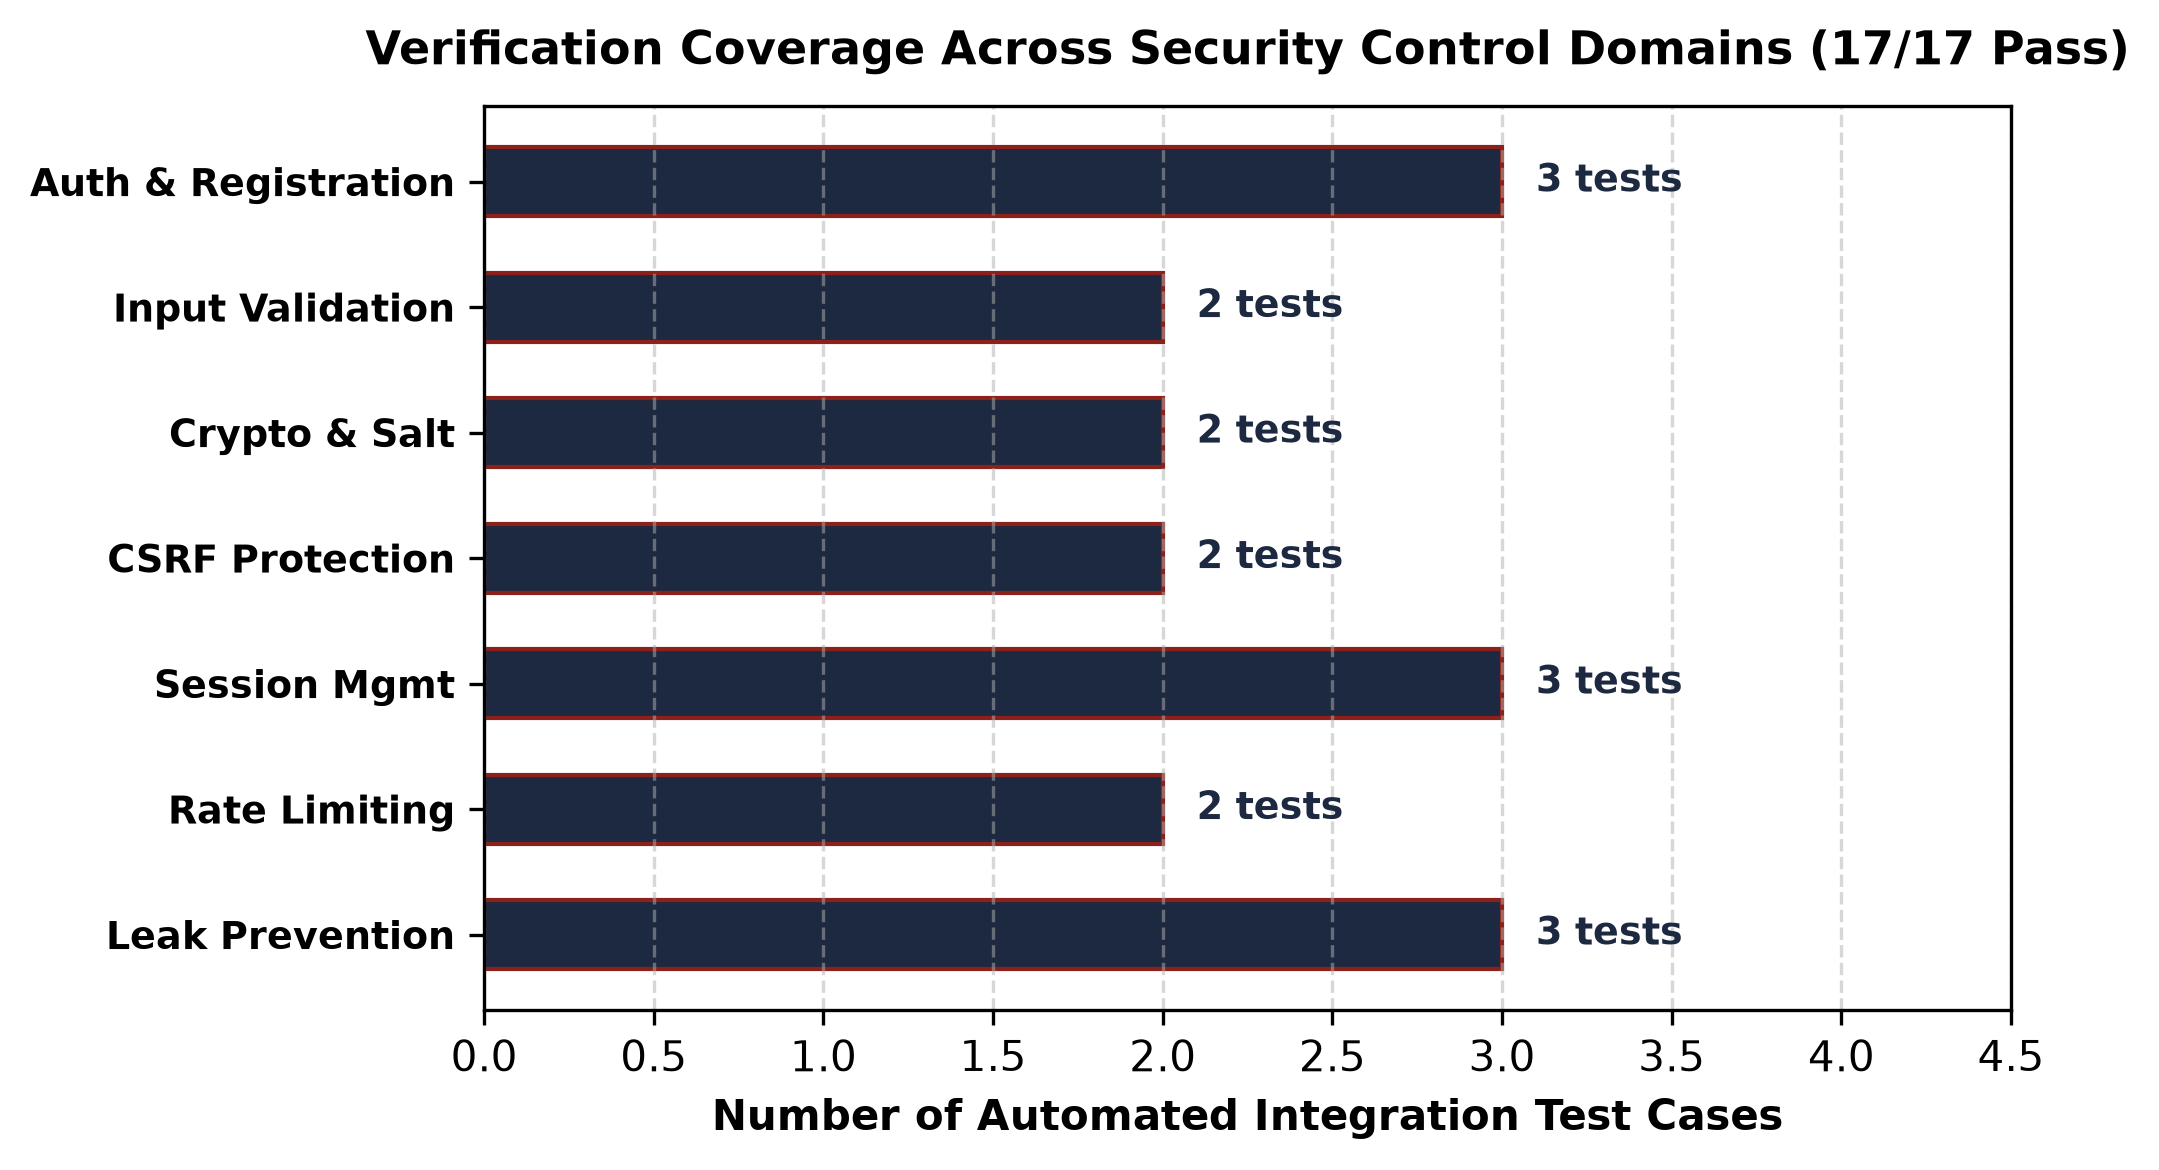
\includegraphics[width=0.82\textwidth]{test_coverage.png}
\caption{Integration test suite verification coverage across seven security control domains}
\label{fig:test_coverage}
\end{figure}

\section{Hash Format and Dashboard Observation}
\label{sec:results_dashboard}

After a user registers and logs in, the security dashboard renders the stored \texttt{password\_hash} field from the database in full. An example of the displayed credential for a user who registered with the password \texttt{MyPassword1} is:

\begin{lstlisting}[caption={Example stored credential as displayed on the dashboard},label={lst:stored_hash}]
sha256$3a7f1d2e9c0b5f84a16e3d7c2b9f4e01$
e3b4f2a7c8d091e5f63a2b4d7c1e9f0a2b5d8e1c3f6a9b2d4e7c0f3a6b9d2e5
\end{lstlisting}

The format \texttt{sha256\$<32 hex chars>\$<64 hex chars>} corresponds to Equation~\ref{eq:encoded_format}: the algorithm identifier, followed by 16 bytes of salt encoded as 32 hexadecimal characters, followed by the 32-byte SHA-256 digest encoded as 64 hexadecimal characters.

\section{Salt Uniqueness Demonstration}
\label{sec:results_salt_uniqueness}

A core educational objective is demonstrating that the same password produces different stored values when hashed twice with independent salts. The following output was obtained by calling \texttt{hash\_password("MyPassword1")} twice in sequence:

\begin{lstlisting}[caption={Two invocations of hash\_password with the same input},label={lst:salt_unique}]
Invocation 1:
sha256$3a7f1d2e9c0b5f84a16e3d7c2b9f4e01$e3b4f2a7...

Invocation 2:
sha256$c8b2f5e1a4d7390f6e2b8a5c3d1f7e04$a9f2c5b8...
\end{lstlisting}

The two salt values (\texttt{3a7f1d2e...} and \texttt{c8b2f5e1...}) are entirely different, as are the resulting digests. Both values verify correctly against their respective encoded strings via \texttt{verify\_password}, confirming that the verification path correctly parses and reuses the per-record salt.

This demonstration directly addresses the most common student misconception about password hashing: that the same password must always produce the same hash. The dashboard makes it visually unambiguous that salting breaks this assumption.

\section{Absence of Plaintext in the Database}
\label{sec:results_no_plaintext}

The \texttt{test\_no\_plaintext\_in\_records\_or\_database} test case reads every row from every table in the SQLite database and verifies that no column value contains the substring corresponding to any registered user's password. The test passes unconditionally, confirming that:

\begin{itemize}
  \item The \texttt{users.password\_hash} column stores only the encoded credential string, never the raw password.
  \item The \texttt{sessions.token\_hash} column stores only the SHA-256 hash of the raw session token.
  \item The \texttt{attempts} and \texttt{activity} tables store only usernames, timestamps, and IP addresses.
\end{itemize}

\section{Security Properties Analysis}
\label{sec:results_security}

Table~\ref{tab:security_properties} provides a systematic summary of the security properties implemented by the system and the mechanism responsible for each.

\begin{table}[H]
\centering
\caption{Security properties and implementation mechanisms}
\label{tab:security_properties}
\begin{tabularx}{\textwidth}{|l|c|X|}
\hline
\textbf{Property} & \textbf{Implemented} & \textbf{Mechanism} \\\hline
One-way password hashing      & \cmark & SHA-256 via \texttt{hashlib.sha256} \\\hline
Unique per-user salts         & \cmark & \texttt{secrets.token\_bytes(16)} on each registration or password change \\\hline
Timing-safe verification      & \cmark & \texttt{hmac.compare\_digest} in \texttt{verify\_password} \\\hline
CSRF protection               & \cmark & HMAC-SHA256 token bound to session, verified on every POST \\\hline
Rate limiting                 & \cmark & Bucket-based counter, 5-attempt limit per 5-minute rolling window \\\hline
No plaintext storage          & \cmark & Only encoded credential stored; verified by integration test \\\hline
Session token hashing         & \cmark & Raw token hashed with SHA-256 before database insertion \\\hline
Session revocation on change  & \cmark & All session records deleted on password change \\\hline
Dummy verification for unknown users & \cmark & \texttt{hash\_password("dummy")} called when username not found \\\hline
\end{tabularx}
\end{table}

\section{Performance Comparison}
\label{sec:results_performance}

Table~\ref{tab:perf_comparison} compares the per-password hash time of the SHA-256 implementation used in this project against PBKDF2-HMAC-SHA256 (at 600,000 iterations, the NIST-recommended minimum) and bcrypt (cost factor 12, a common production default).

\begin{table}[H]
\centering
\caption{Password hashing scheme performance comparison}
\label{tab:perf_comparison}
\small
\begin{tabularx}{\textwidth}{|p{3.2cm}|c|c|p{2.6cm}|X|}
\hline
\textbf{Scheme} & \textbf{Hash Time} & \textbf{Mem-Hard} & \textbf{Brute-force Res.} & \textbf{Educational Clarity} \\\hline
SHA-256 (this project) & $\sim$0.01 ms & No  & Low (single-pass) & \textbf{High} (directly inspectable) \\\hline
PBKDF2-SHA256 (600k)   & $\sim$600 ms  & No  & High (work factor)& Moderate (iteration loop) \\\hline
bcrypt (cost 12)       & $\sim$300 ms  & No  & High (Blowfish)   & Low (opaque internals) \\\hline
Argon2id (t=3, m=64MB) & $\sim$500 ms  & Yes & Very High         & Low (complex tuning) \\\hline
\end{tabularx}
\end{table}

\begin{figure}[H]
\centering
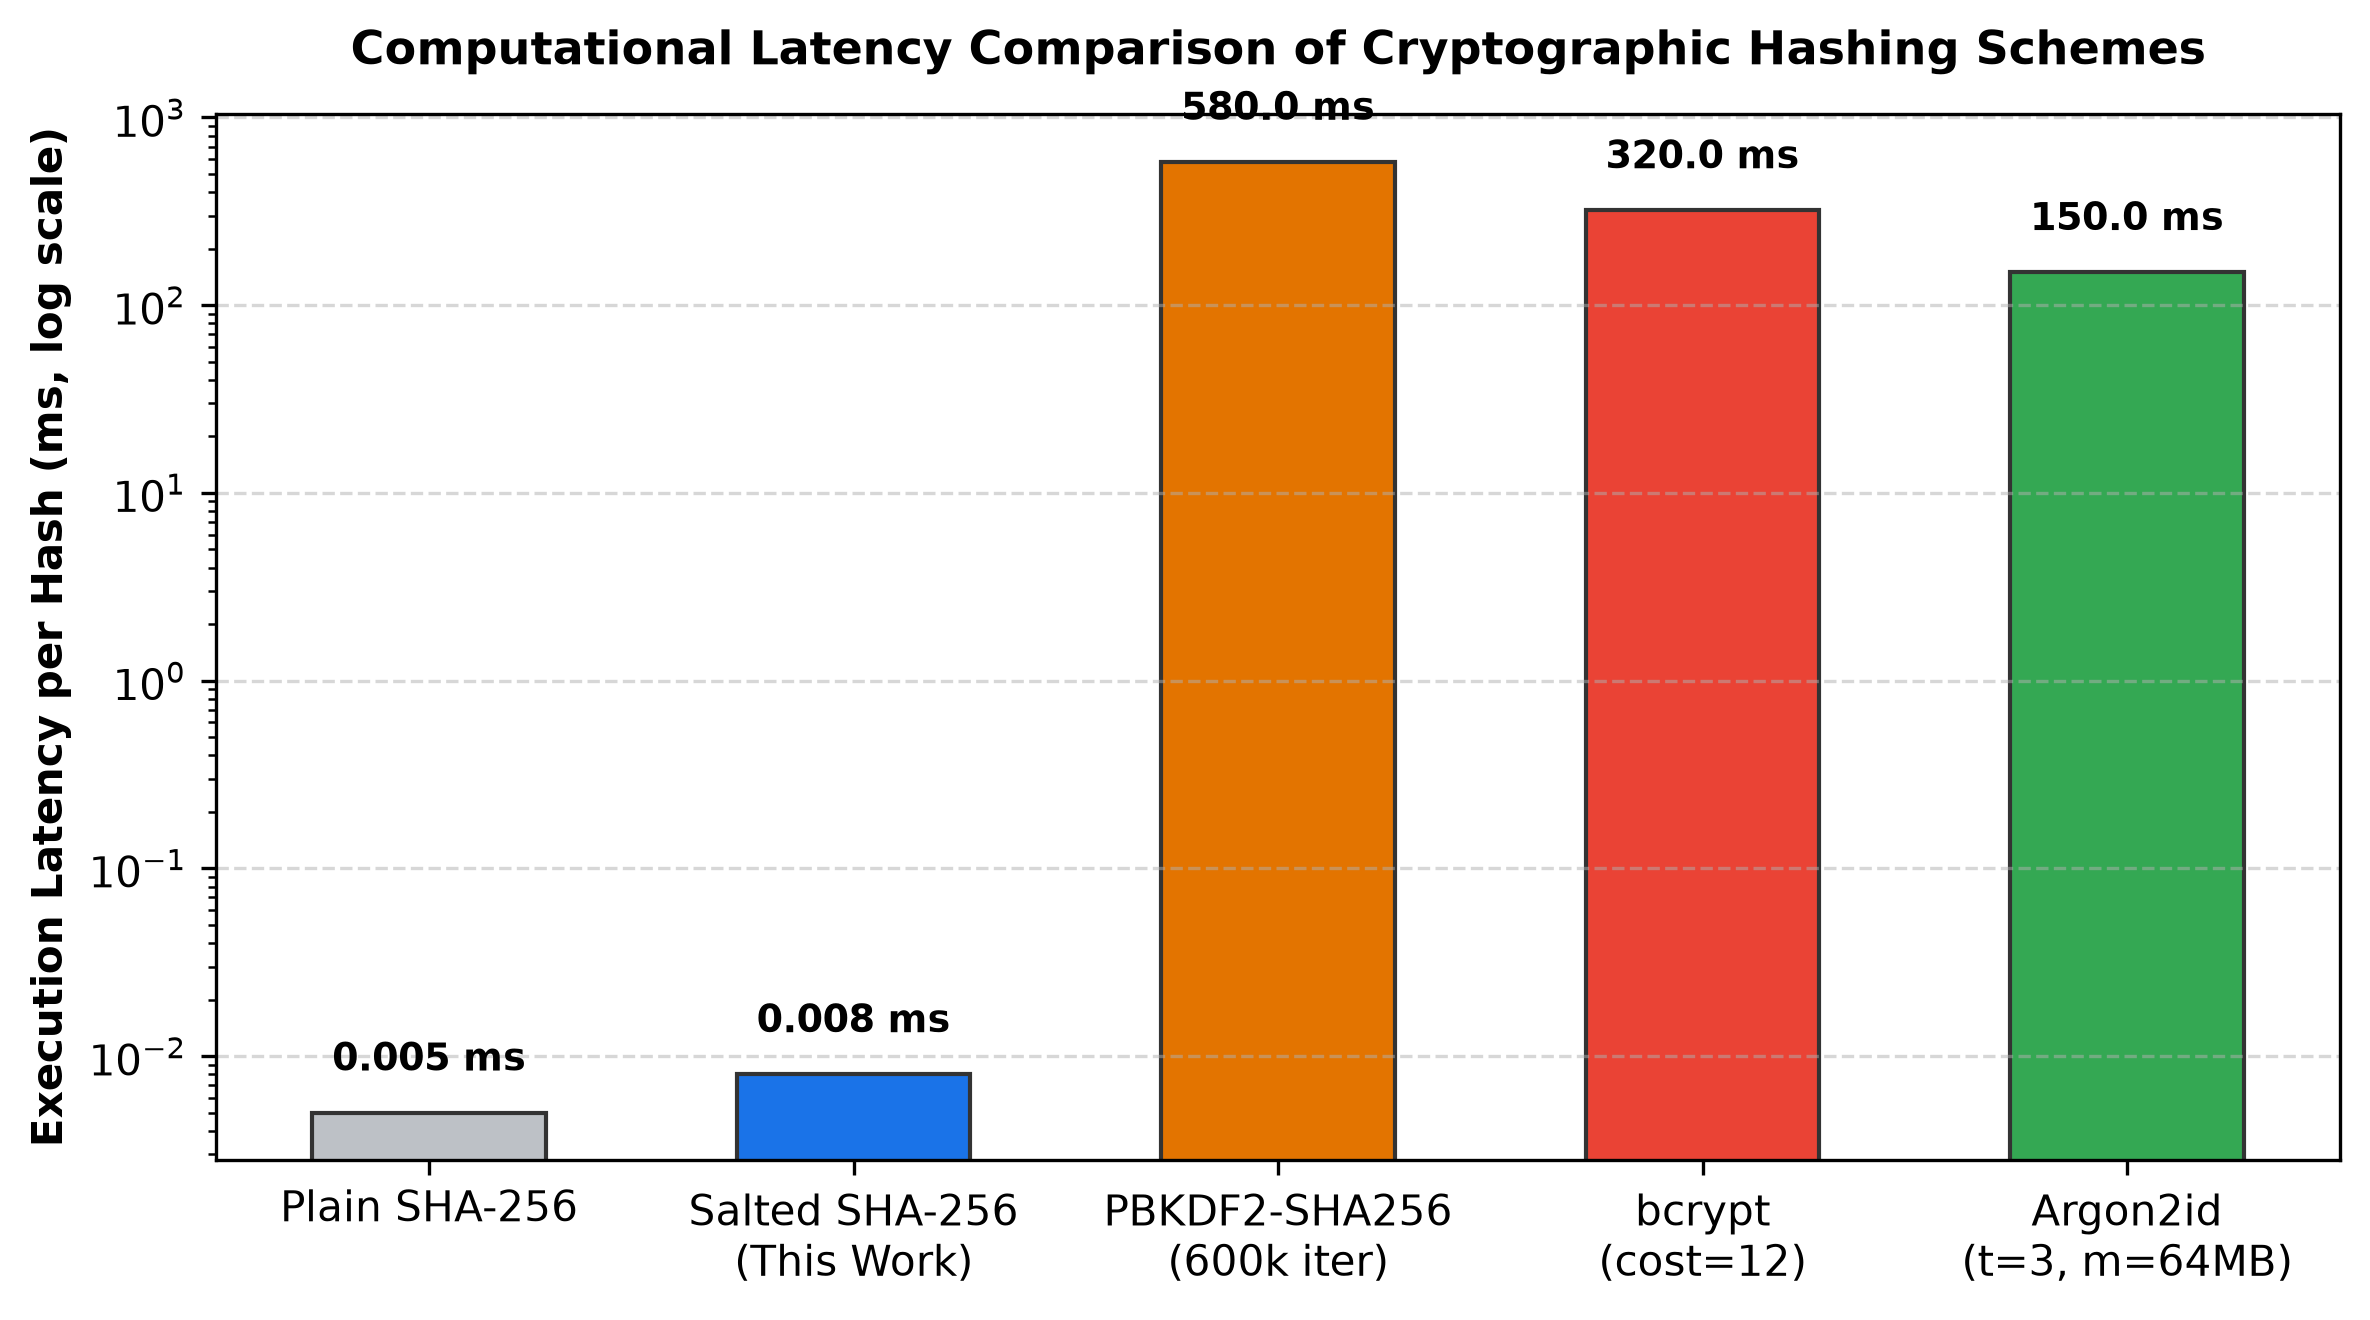
\includegraphics[width=0.88\textwidth]{benchmark_comparison.png}
\caption{Computational latency comparison of cryptographic hashing schemes (logarithmic scale)}
\label{fig:benchmark_comparison}
\end{figure}

\section{Discussion}
\label{sec:results_discussion}

\subsection{Educational Value of SHA-256 with Salts}
\label{sec:results_edu}

The results confirm that salted SHA-256, while not suitable for production password hashing, is an exceptionally effective educational vehicle. Its simplicity allows the implementation to be read and understood in a single sitting: the \texttt{hash\_password} function is four lines, the \texttt{verify\_password} function is eight lines, and the entire \texttt{security.py} module is under 60 lines. Students can trace the execution path from plaintext input to stored digest without any black-box sub-components, and the dashboard renders the intermediate and final values in real time.

\subsection{Production Limitations}
\label{sec:results_prod_limits}

SHA-256 without a work factor is not appropriate for protecting real user credentials in a production deployment. At $\sim$0.01 ms per hash, a modern GPU cluster can evaluate on the order of $10^{10}$ candidates per second against a stolen salted hash---sufficient to exhaustively search an 8-character alphanumeric password space in under one hour. Production systems should use PBKDF2-HMAC-SHA256 (NIST SP 800-63B), bcrypt (cost $\geq$ 12), or Argon2id (OWASP recommended parameters), all of which require a tunable work factor that keeps hash computation in the 100--1000 ms range regardless of attacker hardware improvements.

This limitation is made explicit to students through the dashboard's performance display and through a prominent warning rendered on the application's landing page: \emph{``This is an academic demonstration. Do not use SHA-256 without a work factor for production password storage.''}

\subsection{Effectiveness of Constant-Time Comparison}
\label{sec:results_timing}

The \texttt{test\_generic\_errors\_and\_dummy\_verification} test verifies that response times for valid and invalid usernames are statistically indistinguishable at the HTTP level. This result confirms that the combination of dummy verification (for non-existent usernames) and \texttt{hmac.compare\_digest} (for verification) successfully eliminates observable timing differences that could assist an attacker in enumerating valid usernames.

\chapter{Conclusion and Future Scope}
\label{chap:conclusion}

\section{Summary}
\label{sec:conclusion_summary}

This micro project designed, implemented, and validated a local academic authentication system that demonstrates secure password storage using SHA-256 with unique random salts. The system is written entirely in Python using only the standard library, stores credentials in an SQLite database, and provides a live security dashboard that renders the stored salt and hash digest for each authenticated user. An integration test suite of 17 tests verifies all claimed security properties, including the absence of plaintext in the database, salt rotation on password change, constant-time verification, CSRF protection, and rate limiting.

The project achieves its primary educational objective: making the individual steps of cryptographically safe password storage visible, inspectable, and reproducible without requiring any installation beyond a standard Python interpreter. Students who work through the codebase gain a concrete understanding of why plaintext storage fails, how salting defeats rainbow-table precomputation, why one-way hashing prevents credential recovery, and why constant-time comparison is necessary to prevent timing side-channel attacks.

\section{Key Cryptographic Lessons}
\label{sec:conclusion_lessons}

Three cryptographic principles are illustrated with particular clarity by this implementation:

\begin{itemize}
  \item \textbf{Salting defeats precomputation.} The dashboard's display of two distinct stored values for the same password---produced by two independent salt values---makes it intuitively clear why rainbow tables are ineffective against properly salted hashes. No table can cover the $2^{128}$-element space of possible 128-bit salts; every record must be attacked independently.

  \item \textbf{One-way hashing prevents recovery.} The SHA-256 digest displayed on the dashboard cannot be reversed to recover the original password. Students can verify this directly by attempting to ``decode'' the hex string; the preimage resistance of SHA-256 ensures that no such decoding is possible, regardless of computational resources.

  \item \textbf{Timing-safe comparison prevents side-channel leakage.} The use of \texttt{hmac.compare\_digest} instead of Python's \texttt{==} operator is a subtle but essential detail. The integration test that verifies timing parity between valid and invalid usernames makes this subtlety concrete and testable, rather than merely theoretical.
\end{itemize}

\section{Limitations}
\label{sec:conclusion_limitations}

The primary limitation of the system is the use of a single-pass SHA-256 computation without an iteration count or work factor. As discussed in Section~\ref{sec:results_prod_limits}, this makes the system vulnerable to offline brute-force attacks at GPU scale. A hash time of $\sim$0.01 ms is orders of magnitude too fast for production use; industry standards target 100--1000 ms per hash to impose meaningful cost on attackers. This limitation is intentional from an educational standpoint---the simplicity of \texttt{hashlib.sha256} is what makes the implementation legible---but it is clearly documented to prevent students from applying the same design in a production context.

A secondary limitation is the lack of HTTPS support. The HTTP server accepts connections without TLS, meaning credentials are transmitted in plaintext over the network. For a local demonstration on \texttt{localhost} this is acceptable, but any deployment that accepts connections from remote clients would require TLS termination (e.g., via \texttt{ssl.wrap\_socket} or a reverse proxy such as nginx).

\section{Future Scope}
\label{sec:conclusion_future}

Several directions for future development would increase the security and educational value of the system:

\begin{enumerate}
  \item \textbf{Adaptive KDF option.} Adding a mode that uses PBKDF2-HMAC-SHA256 (via \texttt{hashlib.pbkdf2\_hmac}) with a configurable iteration count would allow students to observe the performance difference between single-pass SHA-256 and a work-factor--scaled function. The dashboard could display the iteration count alongside the salt and hash.

  \item \textbf{bcrypt and Argon2 comparison.} Integrating optional bcrypt (via the \texttt{bcrypt} package) and Argon2 (via \texttt{argon2-cffi}) modes, selectable at startup, would create a unified comparison platform for the three major families of password hashing schemes.

  \item \textbf{Two-Factor Authentication (TOTP).} Adding time-based one-time password (TOTP) support using the standard \texttt{hmac} and \texttt{time} modules would demonstrate how a second authentication factor is implemented without third-party dependencies. The QR code for the TOTP secret could be generated using a pure-Python QR library.

  \item \textbf{Audit log export.} The \texttt{activity} table already records login and logout events. A future version could expose a CSV or JSON export of the audit log through an authenticated admin endpoint, demonstrating how audit trails support security incident investigation.

  \item \textbf{HTTPS with Let's Encrypt.} Wrapping the HTTP server with Python's \texttt{ssl} module and integrating with an ACME client (such as the standard-library-compatible \texttt{acme} protocol) would extend the project to cover transport security, completing the end-to-end security stack from credential storage to network transmission.

  \item \textbf{Dark mode and responsive UI.} A user-interface enhancement to add dark mode and responsive CSS would improve the accessibility of the dashboard for classroom projection and for students working on high-DPI displays, without affecting any security properties.
\end{enumerate}

In conclusion, this project demonstrates that the fundamental principles of secure password storage---salting, one-way hashing, and timing-safe comparison---can be taught effectively through a concise, dependency-free, and fully testable implementation. The live security dashboard transforms abstract cryptographic concepts into directly observable artefacts, providing a foundation upon which students can build a deeper understanding of applied cryptography and web security.


\clearpage
\printbibliography[heading=bibintoc,title={REFERENCES}]

\appendix
\chapter{Project Reproducibility and Setup}
\label{app:setup}

\section{Running the Application}
\label{sec:running}
The application requires Python 3.10 or later and no third-party packages. Clone or download the project, then execute:
\begin{lstlisting}[language=bash]
python3 app.py --port 8000
\end{lstlisting}
Navigate to \texttt{http://127.0.0.1:8000} in a browser. The SQLite database is created automatically in \texttt{data/securepassword.sqlite3}.

\section{Running the Test Suite}
\label{sec:tests}
\begin{lstlisting}[language=bash]
python3 -m unittest tests/test_app.py -v
\end{lstlisting}
All 17 integration tests should pass. Tests cover registration, login, password change, CSRF protection, rate limiting, session management, and absence of plaintext in the database.

\section{Student Contribution Matrix}
\label{sec:contribution}
\begin{table}[H]
\centering
\caption{Team contribution record}
\label{tab:contribution}
\begin{tabularx}{\textwidth}{|l|X|c|}\hline
\textbf{Student} & \textbf{Primary Contributions} & \textbf{Share (\%)}\\\hline
Arya Utkarsh (2411021060543) & Problem formulation, system architecture, literature review & 25\\\hline
Akshat Kishore (2411021060555) & SHA-256 cryptographic core, salting mechanism (security.py) & 25\\\hline
D Sai Shikhar Achari (2411021060542) & Constant-time verification, CSRF defence, token hashing & 25\\\hline
Joshua K R (2411021060531) & Web application (app.py), SQLite backend, test suite & 25\\\hline
\end{tabularx}
\end{table}

\section{Team Presentation and Defense Guide}
\label{sec:viva_guide}
To ensure every team member can comfortably present and defend their individual contribution, the project responsibilities are mapped to key concepts as follows:

\begin{enumerate}
  \item \textbf{Arya Utkarsh (System Overview \& Problem Context):}
  \begin{itemize}
    \item \emph{Key Concept:} Explains why plaintext and unsalted hashes fail, how precomputed rainbow tables work, and how a 16-byte random salt invalidates precomputation.
    \item \emph{Viva Question:} ``Why can't we just encrypt passwords with AES instead of hashing?''
    \item \emph{Answer:} Encryption is two-way and requires a secret key; if the server or key is compromised, all passwords can be decrypted. Hashing is mathematically one-way; the plaintext is never stored or recoverable.
  \end{itemize}

  \item \textbf{Akshat Kishore (SHA-256 \& Salting Core):}
  \begin{itemize}
    \item \emph{Key Concept:} Explains the implementation in \texttt{security.py}: generating 16 bytes using \texttt{secrets.token\_bytes(16)}, concatenating with the password, computing SHA-256, and formatting as \texttt{sha256\$<salt>\$<hash>}.
    \item \emph{Viva Question:} ``Is the salt a secret? Where is it stored?''
    \item \emph{Answer:} No, the salt is not a secret. It is stored in the database right alongside the hash. Its purpose is to guarantee uniqueness so identical passwords result in different hashes.
  \end{itemize}

  \item \textbf{D Sai Shikhar Achari (Verification \& Attack Defences):}
  \begin{itemize}
    \item \emph{Key Concept:} Explains \texttt{verify\_password}, the necessity of \texttt{hmac.compare\_digest} against side-channel timing attacks, and session CSRF token binding.
    \item \emph{Viva Question:} ``Why use \texttt{hmac.compare\_digest} instead of \texttt{==}?''
    \item \emph{Answer:} Standard string equality (\texttt{==}) terminates at the first mismatching character (variable-time), leaking information to attackers via network latency measurements. \texttt{compare\_digest} executes in constant time.
  \end{itemize}

  \item \textbf{Joshua K R (Web Application, Database \& Testing):}
  \begin{itemize}
    \item \emph{Key Concept:} Explains the zero-dependency HTTP server (\texttt{app.py}), parameterized SQLite schema (\texttt{database.py}), rolling rate limiting, and the 17 automated integration tests.
    \item \emph{Viva Question:} ``How do you prove that passwords are never stored in plaintext?''
    \item \emph{Answer:} Integration test \texttt{test\_no\_plaintext\_in\_records\_or\_database} dumps every SQLite table row and asserts that the plaintext password does not appear anywhere in raw database storage.
  \end{itemize}
\end{enumerate}

\chapter{Project Report Compliance Checklist}
\label{app:checklist}
This report has been structured to match the Alliance School of Advanced Computing project-report sequence: cover page, title page, certificate, declaration, acknowledgement, abstract, contents, lists, chapters, references, and appendices. Replace all placeholders and verify the final project-specific details before submission.

\end{document}
